\documentclass[12pt,twocolumn,letterpaper]{article}

\usepackage{statcourse}
\usepackage{times}
\usepackage{epsfig}
\usepackage{graphicx}
\usepackage{amsmath}
\usepackage{amssymb}

% Include other packages here, before hyperref.

% If you comment hyperref and then uncomment it, you should delete
% egpaper.aux before re-running latex.  (Or just hit 'q' on the first latex
% run, let it finish, and you should be clear).
\usepackage[breaklinks=true,bookmarks=false]{hyperref}


\statcoursefinalcopy


\setcounter{page}{1}
\begin{document}


%%%%%%%%%%%%%%%%%%%%%%%%%%%%%%%%%%%%%%%%%%%%%%%%%%%%%%%%%%%%%%%
% DO NOT EDIT ANYTHING ABOVE THIS LINE
% EXCEPT IF YOU LIKE TO USE ADDITIONAL PACKAGES
%%%%%%%%%%%%%%%%%%%%%%%%%%%%%%%%%%%%%%%%%%%%%%%%%%%%%%%%%%%%%%%

%%%%%%%%% TITLE
\title{What are you drawing? Classifying Google Quick, Draw! Doodles}

%我忘记加上了random forest, 你们酌情在需要的地方加一下%

\author{Tong Li\\
{\tt\small tli287@wisc.edu}
\and
Runxin Gao\\
{\tt\small rgao35r@wisc.edu}
\and
Kenny Jin\\
{\tt\small jjin59@wisc.edu}
}

\maketitle

% MAIN ARTICLE GOES BELOW
%%%%%%%%%%%%%%%%%%%%%%%%%%%%%%%%%%%%%%%%%%%%%%%%%%%%%%%%%%%%%%%


%%%%%%%%% ABSTRACT
\begin{abstract}
Image recognition, especially from scratchy and noisy data, plays a significant role in machine learning. In our project we want to classify the hand-drawn doodles, with 345 categories in total, from Google Quick Draw. We construct different algorithms such as the k-nearest neighbors (KNN), Logistic Regression, and Convolutional Neural Network (CNN), and they each obtains an accuracy of {}. We also experimented different dimensionality reduction methods for KNN and Logistic Regression. By comparing model performances, we can gain an insight on which classifier is the most suitable for classifying doodles with a lot of categories.
\end{abstract}

% 要用现在时

%%%%%%%%% BODY TEXT
\section{Introduction}

Quick, Draw!\footnote{https://quickdraw.withgoogle.com/} is an online game released by Google on November, 2016 where the user is prompted with a specific requirement to draw a picture in 20 seconds and the algorithm will make a prediction based on the drawing. Millions of images were collected by Google through this game, and they were utilized to make better and quicker predictions. Figure \ref{fig:quickdraw} showed an example of such images\footnote{https://github.com/googlecreativelab/quickdraw-dataset}. Such large-scale data set leaves many to the imagination of machine learning enthusiasts and encourages the rises of creative projects. For example, Quartz has explored the drawing habits like stroke order grouped by different countries and found clear associations between the drawing and their language styles \cite{quartzcircle}; others tried several different prediction models evaluated by prediction accuracy \cite{github}.

More than simply classifying doodles, such algorithms could have educational applications for language-learning toddlers as well. They can draw what they see, and learn how to spell or say it, which could accelerate the language learning process. Moreover, since doodles are somewhat sketchy, by constructing algorithms that can make accurate predictions based on sketchy images, the uses of the algorithms could be extended to convert handwritten text to computer, eliminating the need to type all the words.

In our project, rather than building separate algorithms for each category or subset of categories, we combined all categories together as our data set. Therefore, since our data set has 345 categories in total, the prediction accuracy is not very high, but is still higher than what we expected. We apply several algorithms such as KNN, Logistic Regression and CNN, and adopt different variations of dimension reduction methods.

\begin{figure}[ht]
\begin{center}
   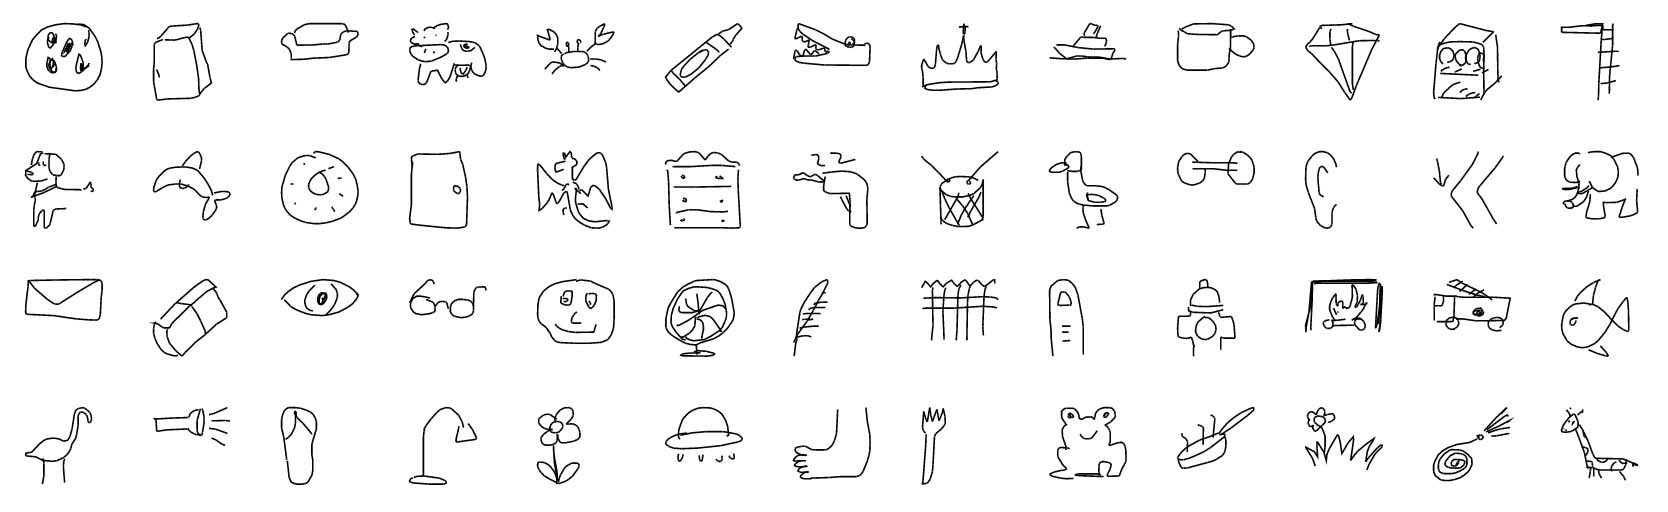
\includegraphics[width=1\linewidth]{figures/quickdraw_image.jpg}
\end{center}
   \caption{Example of quick draw images}
\label{fig:quickdraw}
\end{figure}


\begin{figure}[ht]
\begin{center}
   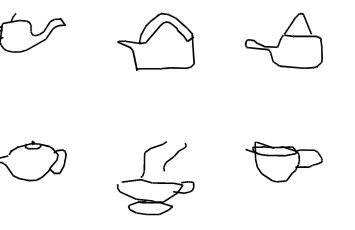
\includegraphics[width=0.8\linewidth]{figures/teapot.png}
\end{center}
   \caption{Example drawings of teapot}
\label{fig:teapot}
\end{figure}

\section{Related Work}

Quick, Draw! dataset is popular among machine learning enthusiasts once it has been released. Similar to our tasks, many experts of machine learning compared different classification algorithms to recognize doodles. Harun-Ur-Rashid experimented on the dataset in the Kaggle competition [1]. He applied six machine learning algorithms: KNN, Random Forest,  Linear Support Vector Clustering (SVC), Gaussian Radial Basis Function SVC, Multi-Layer Perceptron, and CNN. His goal was to classify doodles into only two categories and to analyze the performances of these models. When Harun-Ur-Rashid obtained relatively high classification acccuracies of all models, we attempt to classify doogles into 345 categories which are all categories of the original dataset and to check whether algorithms can remain consistently high accuracies. 

Guo, WoMa, and Xu experimented three algorithms on the dataset: 1-Closest Centroid (1-CC),  KNN with K-Means++, and CNN to classify doodles into all 345 unique categories [2]. They set the accuracy of 1-CC as the baseline and compared the model performances of KNN and CNN. They obtained the accuracies of 23.6\%, 34.4\% and 62.1\% respectively; therefore, they concluded that CNN outperformed than other two algorithms. Surprised by the advantages of CNN on computer vision, we further explore two CNN models to see how CNN model can perform at the best for the computer vision prombles; so we tried two kinds of CNN models: LeNet-5 and ResNet-34 and tuned their parameters. 

Besides, there are some creative explorations on the dataset. For example, Ha and Sonnad used the public database from Quick, Draw! to find relations between the styles of drawing basic shapes and major language groups.They found that the drawing stroke orders were highly influenced by the languages and cultures. Inspired by their amazing conclusions, we try to use another machine learning algorithm mini-batch K-means Clustering to explore the similarities of drawing styles among all 345 distinct categories of distinct doodles. 





\section{Proposed Method}

The data we have in hand is in the general form of typical image data, with 784 dimensions, each representing a pixel of the image. When firstly look at out data, we find the data has a bunch of uninformative features, i.e. the dataset have a lot of features with value zero for all images. Therefore, we decided to apply dimensionality reduction methods to get rid of such unuseful features and to improve computational efficiency. 

We start building the classifier with KNN, which is a lazy algorithm that does not learn from the data but simply memorize. We then fit the data into penalized multinomial logistic regression with cross-validation. Then we use Support Vector Machine as well as Convolutional Neural Network as somehow more 'advanced' tools to classify the doodles. We define the accuracy score by the proportion of the number of doodles correctly classified.

$$ACC = \frac{\text{Number of Correctly Classified}}{\text{Total number of Doodles}}$$

We randomly split our data into 80\% training and 20\% testing.

\subsection{k-Nearest Neighbors}

The first method that comes in mind when doing classification tasks is the k-Nearest Neighbors algorithm. It is a lazy algorithm that simply memorize the data. KNN algorithms takes two parameters: k, the number of neighbors to be considered, and p, the parameter for the Minkowski distance function. Minkowski distance is defined as
$$D(\mathbf{X}, \mathbf{Y}) = (\sum_{i = 1}^{n} (\lvert x_i - y_i \rvert)^p)^\frac{1}{p}$$
And this distance corresponds to the Manhattan Distance when p = 1, and Euclidean Distance when p = 2.
 
When classifying a data point, KNN calculates the k nearest neighbors by the Minkowski distance defined by p, get their labels, and then determine the label of the new data through majority (or plurality) voting. To obtain the optimal k, we conduct 5-fold cross validation on the training set. To wit, the training set is split into 5 portions, and the algorithm is fit five times. Each time the KNN use 4 portions as training and the remaining one as validation. The final accuracy is obtained by averaging the performance of the 5 validation sets in each fitting. In addition, since KNN can be susceptible to the curse of dimensionality, we apply two dimensionality reduction methods: Principal Component Analysis and Autoeocoder.  %可以加一个5-foldcv的图%  , %介绍一下PCA 和 AE%
The number of optimal components is also obtained through cross-validation. The number of hidden layers in Autoencoder is the same as PCA's number of components. 

\subsection{Multinomial Logistic Regression}

We then fit the data into multinomial logistic regression with L1 penalty (LASSO). %加一个feature_selection里那个L1的图%
Multinomial logistic regression returns the probability of the label equals to k with the following equation
$$\mathbf{Pr}(Y^{[i]} = k) = \frac{e^{\beta_k \mathbf{X}^{[i]}}}{\sum_{i = 1}^{K} e^{\beta_i} \mathbf{X}^{[i]}}$$

To prevent this model from overfitting the data, we apply L1 penalty to the model, with coefficient $\lambda$ obtained through 5-fold cross validation. We also use the two dimensionality reduction methods as mentioned above to accelerate computational time. 

\subsection{Random Forest}

\subsection{Convolutional Neural Network}

Describe the method(s) you are proposing, developing, or using. I.e., details
of the algorithms may be included here. 

\section{Experiments}


\subsection{Dataset}

The original data set we have consists of 345 Numpy Bitmap files from Google, each .npy consists of thousands of gray scale images for each category. Google has already preprocessed the data in .npy files by only keeping image data and centering the image with 28 * 28 pixels. Because it is not practical to run the whole data set on our computer, we decide to take a random sample of 1000 images from each category, and combined them to one single .npy file, which has 345,000 images in total. In fitting the models, we split our data set as 80\% for training and 20\% for testing using $train_test_split$ in Sci-Kit Learn stratified on labels. Each image is represented as having 784 dimensions, with values representing the intensity of each pixel, ranging from 0 - 255. We apply max-min normalization to the image data, and the range thus becomes 0 - 1. In addition, the label is represented as 0 - 344 for each category, rather than the exact text label. Global random seed is set at 123.

\subsection{Dimensionality Reduction}

\paragraph{PCA}
Since image is centered, we find that there are a lot of features that are all zeroes for all images, thus making them uninformative in model prediction. Therefore, we decide to use Principal Component Analysis to get rid of uninformative features and reduce dimensions. We firstly graphed the explained variance of the feature %加pca那个图%,
we find that 256 features already explain 100\% of the variance in the data, and that there does not seem to be a much difference between 100, 200, and 256. Thus we apply cross-validation to find the optimal number of components for KNN and \texttt{n\_component} = 100 is suggested. We fit the PCA on training set, and transform training and test sets to be of 100 dimensions.

\paragraph{Autoencoder}
We also applied another method of dimensionality reduction called autoencoder. Since PCA is only an linear method, we are concerned that it may not preserve the information in the images very well. On the contrary, the method of autoencoder might perform better than PCA regarding the task of dimensionality reduction. The autoencoder we used for this project is a 3-layer neural network, with one input layer, one hidden layer and one output layer. The input layer takes in the original image vector with 784 dimensions, and the output layer reconstructs the image back to 784 dimensions. We set the number of nodes in the hidden layer to be 100 to make it consistent with PCA. We set the learning rate as 0.05, the random seed as 123 and the batch size as 1000. After 15 epochs of training, the autoencoder can already reconstruct the images pretty well. Then we rerun the autoencoder on all the examples (1000 images for each category) and extracted the hidden layer vectors (100 dimensions) as a new dataset whose dimension was reduced.
%Add original images and images reconstructed from autoencoder%

%parameter settings(epoch, rate 之类的), details, graph前后对比, num_hidden = 100 because pca = 100 to make consistent. %

\subsection{k-Nearest Neighbors}

To obtain the optimal choice of k and \texttt{n\_components}, we use the GridSearchCV function with 5-fold cross validation. We make a pipeline to determine the combination. For PCA the number of components to be chosen from are [100, 200, 256], and for k the range is [5,100] with step = 5. Since our data set is too large and GridSearchCV failed to return the result even after one and a half days, we decided to run it on a smaller subset with 200 images for each category. This greatly enhanced the computational time. We then use Autoencoder to compress the data into smaller dimensions and fit the kNN model with optimal k obtained previously, and compare the results. We abort training kNN with full dimensions after the computation takes more than one day.

\subsection{Multinomial Logistic Regression}

Because we have so many features in our data, we use L1 penalization for the logistic regression to avoid overfitting of the data. We adopt the 5-fold cross validation to determine the optimal strength of penalty $(\lambda)$. %可以在详细介绍一下这个penalty,不用说具体得到的parameter。 得出来的parameter可以放到results里, 这里就重点讲一下怎么去得到%。

We fit the model with three different training sets: one with dimensions reduced by PCA, one with dimensions reduced by Autoencoder, and one with full 784 dimensions to compare model performance. As suggested in Sci-Kit Learn's documentation, we choose SAGA as our solver. We also change the tolerance level to 0.05 because the default tolerance makes it extremely slow for the model to converge.

\subsection{Random Forest}

\subsection{Convolutional Neural Network}




\section{Results and Discussion}

\begin{table}
\begin{center}
\begin{tabular}{|l|c|}
\hline
Model & Accuracy \\
\hline\hline

\text{KNN\_PCA100} &  33.19 \% \\
\text{KNN\_Autoencoder} &  26.13 \% \\
\text{Logistic\_PCA100} & 24.67 \% \\
\text{Logistic\_Autoencoder} & 23.72 \% \\
\text{Logistic\_784} & 23.96 \% \\
\text{Random Forest} & fill \% \\
\text{CNN\_LeNet5} & 47.25 \% \\
\text{CNN\_ResNet34} & 59.96 \% \\
\hline
\end{tabular}
\end{center}
\label{tab:accuracy}
\caption{Test Set Accuracy for Different Models}
\end{table}

For KNN, the optimal combination is \texttt{n\_components} = 100 and k = 15. Therefore when using autoencoder, we also compress the data into 100 dimensions. For logistic regression, three models actually have different penalty strength. The optimal penalty strength returned by LogisticRegressionCV is 100, 10000, and 1 for PCA-100, Autoencoder-100 and full dimensions, respectively. Table \ref{tab:accuracy} shows the test set accuracy we obtain from each model.

\subsection{k-Nearest Neighbors}

By adopting GrivSearchCV on a subset of the training data, the optimal number of neighbors to be considered is 15, and the best number of components is 100. By reducing the data into 100 dimensions using PCA and Autoencoder, prediction accuracy on test set is 33.19 \% and 26.13\% respectively. Because we have too many data with large dimensions, KNN takes several hours to be trained. The discrepancy of the test set accuracy is quite large for different dimensionality reduction methods.

\subsection{Multinomial Logistic Regression}

By training the logistic regression with their optimal L1 penalty strength obtained from cross-validation, the test accuracy is 24.62\%, 23.72\%, 23.96\% for PCA-100, Autoencoder-100, and full dimensions. The test set accuracy is not quite different for these three models, but it takes much less time to fit the regression with reduced dimensions.


\subsection{Random Forest}


\subsection{Convolutional Neural Network}

\subsection{Discussion}

As expected, CNN returns the best test set accuracy for doodle classification, while logistic regression does not perform so well. %加一些解释%
By looking at the discrepancy between training accuracy and test set accuracy, we see that for each model overfitting occurs.
%第二段可以写limitations%
%limitations: auto encoder different compression may be better (或者different hyperparameters, 因为调参太慢了) / gridsearchcv knn的时候jump的太多了(一次五步), 可以试试小一点的jump%
%Logistic Regression 没有cv pca, 所以可能别的pca value更合适%
%因为category太多, data看起来不够多, 如果更多data应该会提高%
%现在的0-1 loss function太严厉了, 可以给missclassified but similar categories some partial credits%
%等等%

\section{Explore drawing styles using mini batch K-Means Clustering}
\subsection{Methodology}
We choose K-means Clustering group pictures of their characteristics considering expensive computational cost of K-means Clustering. Then we use the Elbow method select the optimal hyperparameter K. From Figure 3, we choose 50 clusters since the distortion is dramatically decreasing after 50 clusters. 

\begin{figure}[ht]
\begin{center}
   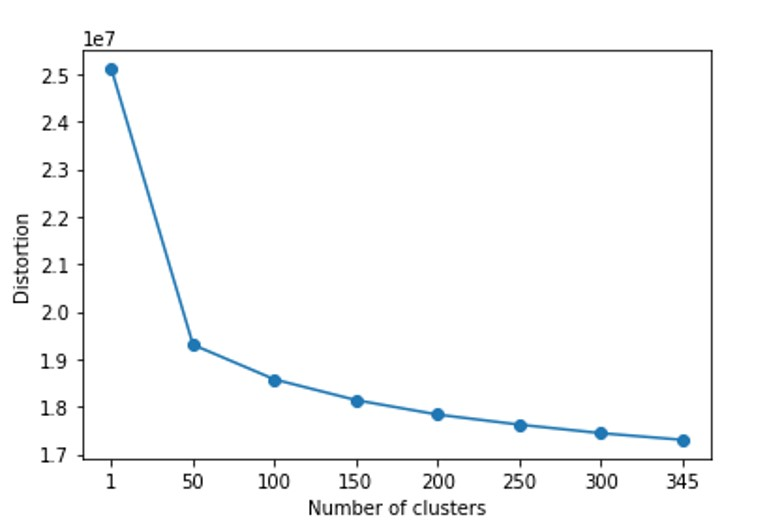
\includegraphics[width=1\linewidth]{figures/K_means_clustering.jpg}
\end{center}
   \caption{Distortions with each number of clusters }
\label{fig:quickdraw}
\end{figure}

\subsection{Discussion}
We found that the top 10 categories of drawing with most similar drawing styles are "line," "headphones," "rainbow," "pear," "triangle," "t-shirt," "The Eiffel Tower," "rifle," "tennis racquet," and "wine glass." These categories basically are common in daily life and usually have simpler shapes so that people tend to agree with each other on how to 

\begin{figure}[ht]
\begin{center}
   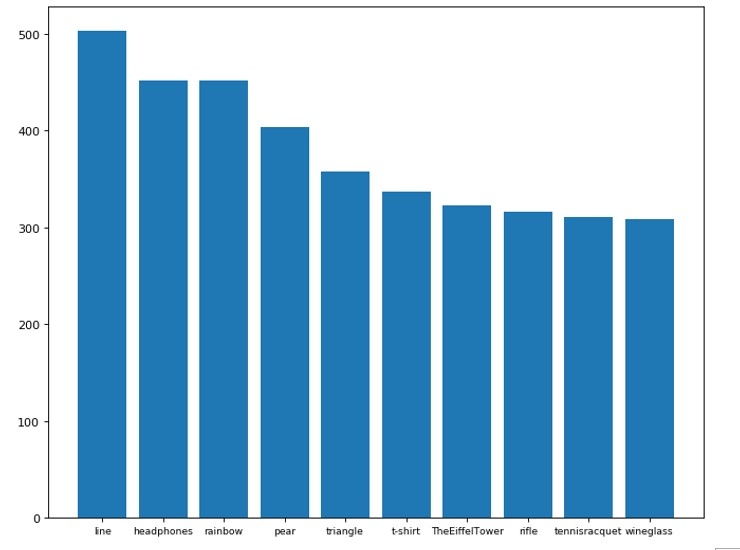
\includegraphics[width=1\linewidth]{figures/top_category.jpg}
\end{center}
   \caption{Top 10 categories among all clusters}
\label{fig:quickdraw}
\end{figure}


\begin{figure}[ht]
\begin{center}
   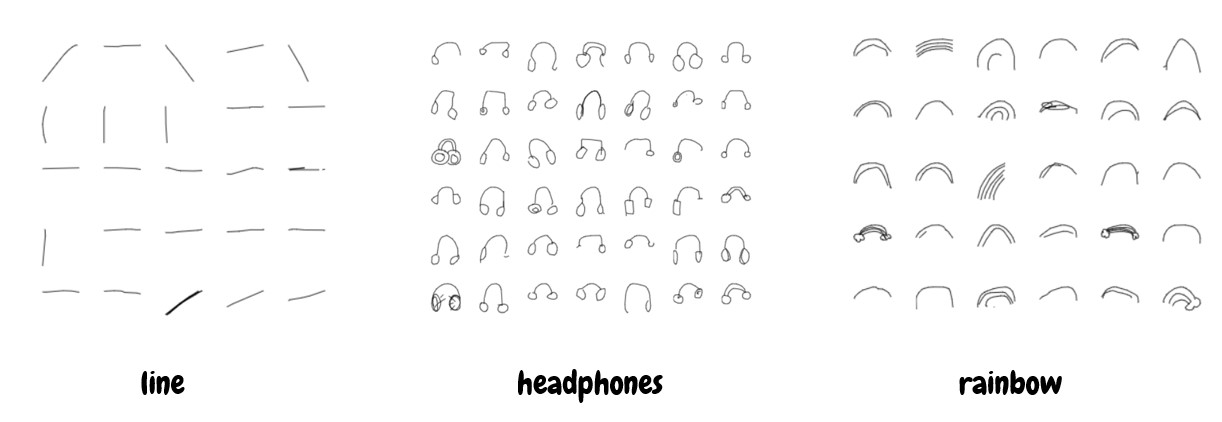
\includegraphics[width=1\linewidth]{figures/1.jpg}
\end{center}
   \caption{Examples of }
\label{fig:quickdraw}
\end{figure}


\begin{figure}[ht]
\begin{center}
   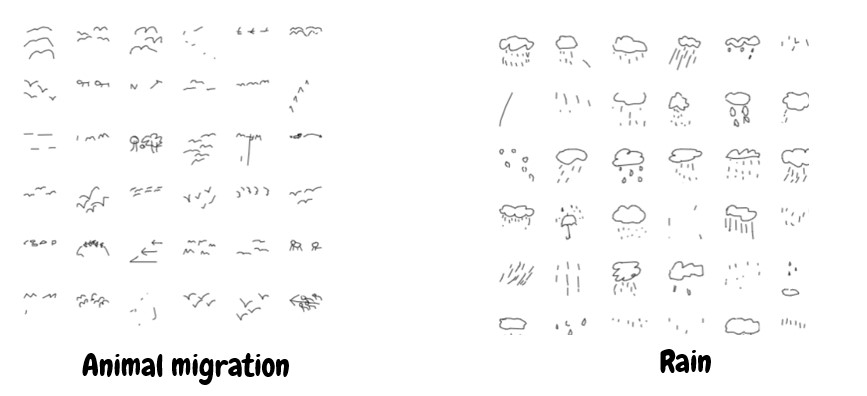
\includegraphics[width=1\linewidth]{figures/2.jpg}
\end{center}
   \caption{Examples of }
\label{fig:quickdraw}
\end{figure}

\begin{figure}[ht]
\begin{center}
   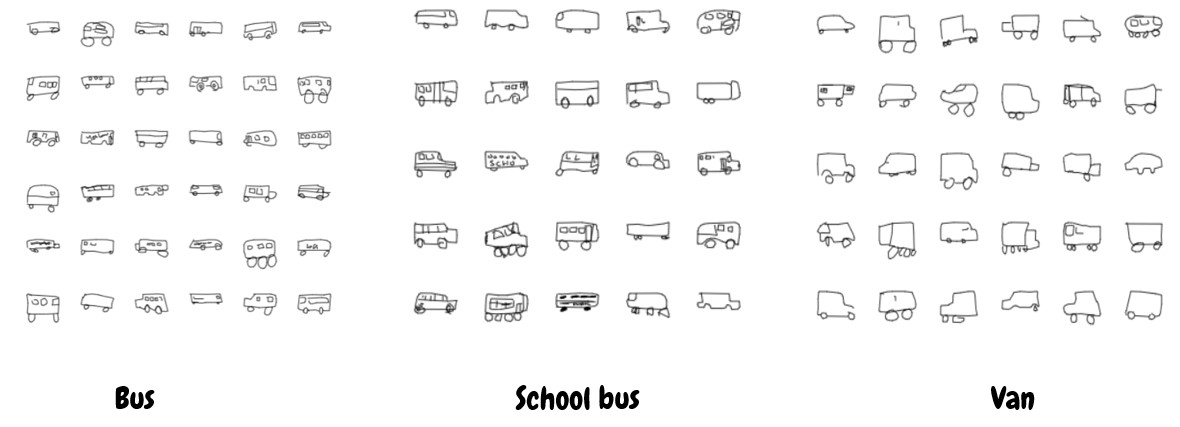
\includegraphics[width=1\linewidth]{figures/3.jpg}
\end{center}
   \caption{Examples of }
\label{fig:quickdraw}
\end{figure}

\begin{figure}[ht]
\begin{center}
   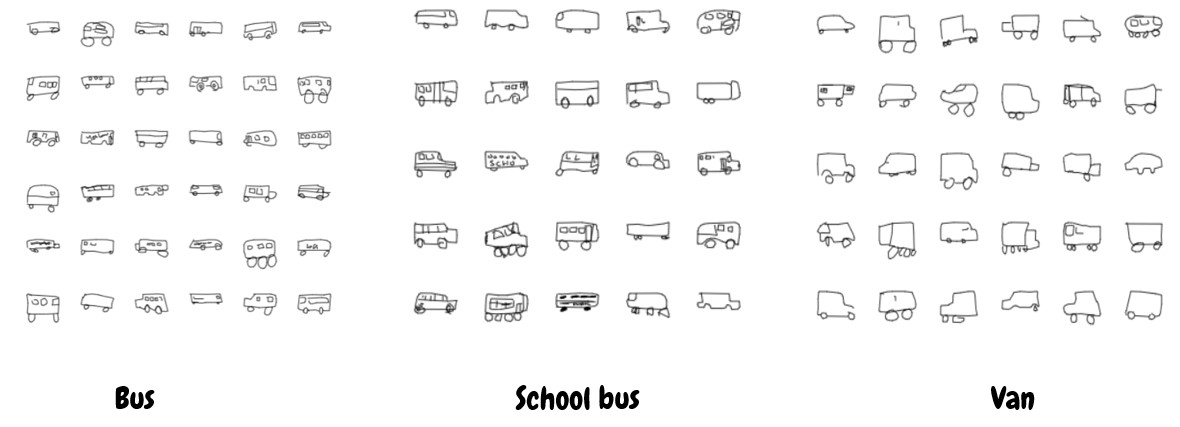
\includegraphics[width=1\linewidth]{figures/3.jpg}
\end{center}
   \caption{Examples of }
\label{fig:quickdraw}
\end{figure}


\begin{figure}[ht]
\begin{center}
   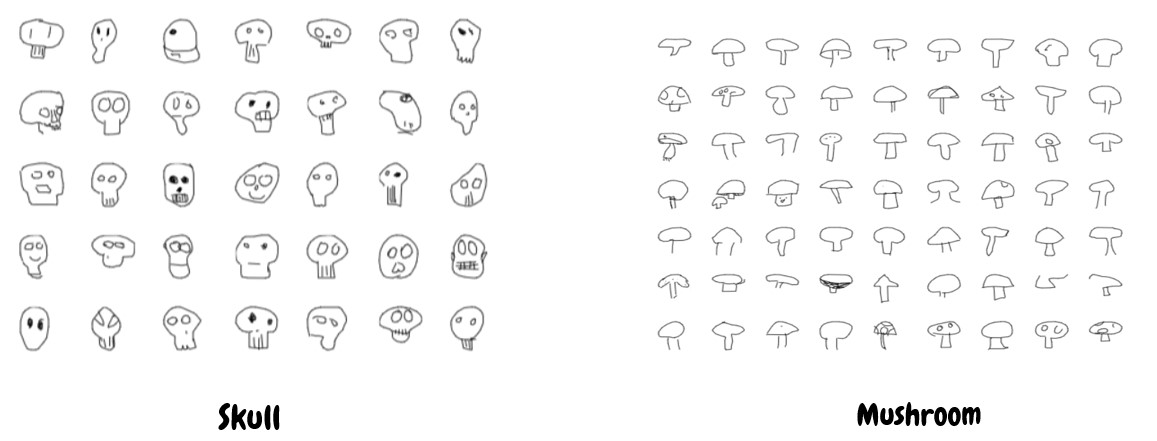
\includegraphics[width=1\linewidth]{figures/4.jpg}
\end{center}
   \caption{Examples of }
\label{fig:quickdraw}
\end{figure}


\begin{figure}[ht]
\begin{center}
   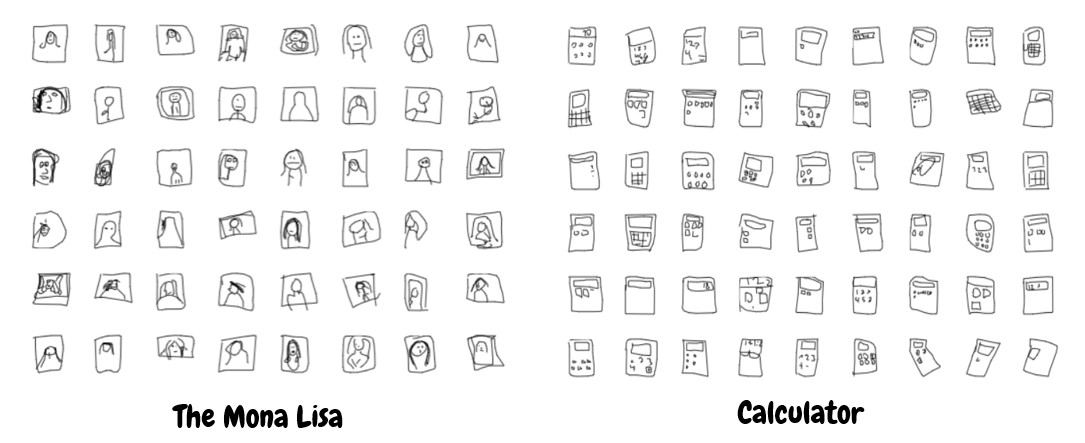
\includegraphics[width=1\linewidth]{figures/5.jpg}
\end{center}
   \caption{Examples of }
\label{fig:quickdraw}
\end{figure}

\begin{figure}[ht]
\begin{center}
   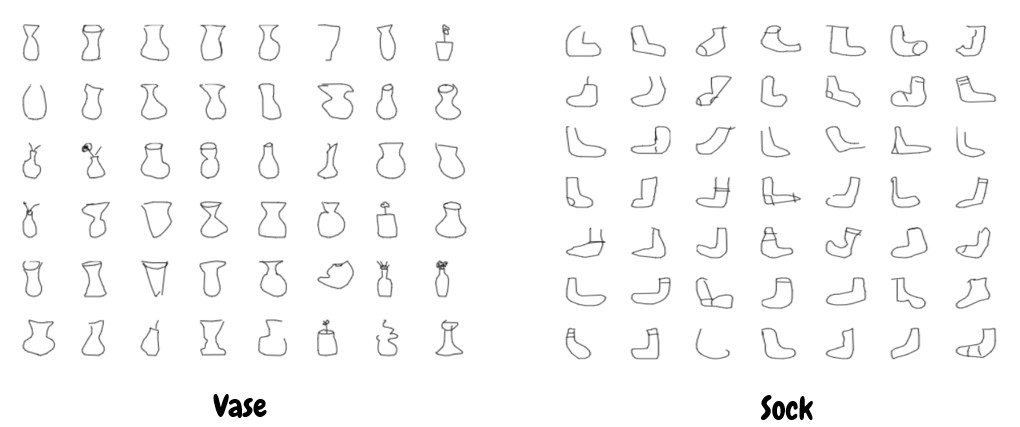
\includegraphics[width=1\linewidth]{figures/6.jpg}
\end{center}
   \caption{Examples of }
\label{fig:quickdraw}
\end{figure}





\section{Conclusions}



Describe your conclusions here. If there are any future directions, you can
describe them here, or you can create a new section for future directions.

\section{Acknowledgements}

%include ae and cnn code source (赛老师的)
We would like to express our thanks to Prof. Raschka for kindly providing us with suggestions about this project and code examples for the implementations of CNNs.

\section{Contributions}

Each group member contributed evenly to data cleaning, modeling, and writing of this final report.

\section{References}
[1]: Rashid, H. Retrived from https://www.kaggle.com/harunshimanto/lets-play-with-quick-draw.

[2]:Guo, K., WoMa, J., Xu, & E. Quick, Draw! Doodle Recognition. Retrieved from http://cs229.stanford.edu/proj2018/report/98.pdf.

[3]: Sonnad, N. (2017, June 15). How do you draw a circle? We analyzed 100,000 circles to show how culture shapes our instincts. Retrieved from https://qz.com/994486/the-way-you-draw-circles-says-a-lot-about-you/.


{\small
\bibliographystyle{ieee}
\bibliography{bibliography}
}

\end{document}
